\documentclass{standalone} 

\usepackage{tikz}
\usetikzlibrary{arrows.meta,shapes, calc, fit, patterns, positioning, intersections, 3d, matrix, angles, quotes, backgrounds}

\begin{document}

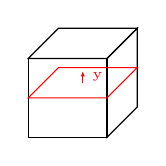
\begin{tikzpicture}

    \tikzset
    {
        font={\fontsize{1pt}{1}\selectfont}
    }

    \pgfmathsetmacro{\cubex}{1}
    \pgfmathsetmacro{\cubey}{1}
    \pgfmathsetmacro{\cubez}{1}
    \draw[] (0,0,0) -- ++(-\cubex,0,0) -- ++(0,-\cubey,0) -- ++(\cubex,0,0) -- cycle;
    \draw[] (0,0,0) -- ++(0,0,-\cubez) -- ++(0,-\cubey,0) -- ++(0,0,\cubez) -- cycle;
    \draw[] (0,0,0) -- ++(-\cubex,0,0) -- ++(0,0,-\cubez) -- ++(\cubex,0,0) -- cycle;

    \draw[red] (0,-0.5,0) -- ++(-\cubex,0,0) -- ++(0,0,-\cubez) -- ++(\cubex,0,0) -- cycle;
    \draw[-{Latex[length=2]},red] (-0.5,-0.5,-0.5) -- node[anchor=west]{y} (-0.5,-0.35,-0.5);

\end{tikzpicture}

\end{document}
